\section{波动率区间预测结果分析与检验}

在前一章中，主要从点预测角度比较了 HAR、GARCH(1,1)、XGB-Market、XGB-AR以及XGB-MIDAS-EPU-DEC五类模型的样本外预测表现。点预测能够反映模型对未来波动率条件水平的刻画能力，但在金融风险管理、资产配置和极端风险预警场景中，仅报告点预测值是不充分的。原因在于，投资者和风险管理者不仅关心未来波动率的条件均值或条件中位水平，也关心预测误差可能处于何种范围之内。因此，在点预测结果之外，进一步构造预测区间能够更完整地评价模型对未来不确定性的刻画能力。

预测区间评价需要同时考虑两个维度：一是区间能否覆盖真实观测值，即有效性；二是在满足合理覆盖率的前提下，区间是否足够窄，即有效性约束下的精确性。若区间过宽，即使覆盖率较高，其实际风险管理价值也有限；若区间过窄，则可能频繁低估真实波动风险。因此，本文在五类点预测模型的基础上，进一步采用滚动共形预测方法构造波动率预测区间，并从经验覆盖率、平均区间宽度、区间得分以及滚动覆盖率等角度对模型进行比较。

本章检验修订DEC是否改善XGB-Market与XGB-AR的区间质量，不预设点预测中的部分指标优势会传递到预测区间。

\subsection{滚动共形预测方法}

本文采用基于历史预测残差的滚动共形预测方法构造区间。共形预测的基本思想是利用校准样本中的预测误差分布，对未来点预测值进行非参数修正，从而得到具有经验覆盖含义的预测区间。经典共形预测方法具有分布无关的优点，在独立同分布或可交换性假设下可以提供有限样本覆盖保证 \citep{Vovk2005,ShaferVovk2008,Lei2018}。然而，金融时间序列通常存在自相关、波动聚集和分布漂移，严格的可交换性假设难以满足。因此，本文不对金融时间序列下的共形区间作过强的有限样本精确覆盖声明，而是将其作为一种按保存预测的日期顺序进行校准的经验区间构造方法；这不验证上游点预测输入的实时可得性。

具体而言，设某一模型在时点 \(t-1\) 对 \(y_t\) 的点预测为 \(\hat{y}_{t|t-1}\)，则预测残差为
\begin{equation}
	e_t = y_t - \hat{y}_{t|t-1}.
\end{equation}
本文采用绝对误差作为非符合度分数：
\begin{equation}
	s_t = |e_t|.
\end{equation}

对于测试集中的任一预测时点 \(t\)，本文仅使用验证集残差和已经实现的历史测试集残差作为校准样本，并取最近 \(m\) 个非符合度分数计算经验分位数。设滚动校准窗口为 \(\mathcal{C}_t\)，其样本量为 \(n_t\)，则 \(1-\alpha\) 预测区间所需的共形分位数为
\begin{equation}
	q_{1-\alpha,t}
	=
	s_{\left(\lceil (n_t+1)(1-\alpha)\rceil\right)},
\end{equation}
其中 \(s_{(k)}\) 表示将校准窗口内非符合度分数从小到大排列后的第 \(k\) 个顺序统计量。若 \(\lceil (n_t+1)(1-\alpha)\rceil>n_t\)，代码将阶数截断至样本量并取最大分数；此做法不提供一般覆盖保证，本实验的窗口与显著性水平不触发这一边界。

在对数波动率尺度上，模型的一步超前预测区间定义为
\begin{equation}
	\left[
	L^{(y)}_{t+1|t},
	U^{(y)}_{t+1|t}
	\right]
	=
	\left[
	\hat{y}_{t+1|t}-q_{1-\alpha,t},
	\hat{y}_{t+1|t}+q_{1-\alpha,t}
	\right].
\end{equation}

本文采用滚动校准而非固定校准，主要基于两点考虑。第一，金融市场波动率的误差分布具有明显时变性，固定校准窗口可能无法及时反映近期市场状态。第二，滚动校准仅使用预测时点之前的近期误差信息，能够在经验上缓解时间序列非平稳性对共形覆盖的影响。类似地，已有时间序列共形预测研究也强调需要对动态序列中的依赖性和分布变化进行适应性处理 \citep{XuXie2021}。

\subsection{区间预测评价指标}

本文从经验覆盖率、平均区间宽度和区间得分三个角度评价预测区间质量。

首先，经验覆盖率定义为
\begin{equation}
	CP_{1-\alpha}
	=
	\frac{1}{N}
	\sum_{t=1}^{N}
	\mathbf{1}
	\left\{
	L^{(y)}_{t+1|t}
	\leq
	y_{t+1}
	\leq
	U^{(y)}_{t+1|t}
	\right\},
\end{equation}
其中 \(N\) 表示测试集评价样本量。经验覆盖率接近名义覆盖率 \(1-\alpha\) 是样本校准表现；需结合抽样误差、违约依赖与其他设置检验，不能单独据此证明区间有效。

其次，平均区间宽度定义为
\begin{equation}
	AW_{1-\alpha}
	=
	\frac{1}{N}
	\sum_{t=1}^{N}
	\left(
	U^{(y)}_{t+1|t}
	-
	L^{(y)}_{t+1|t}
	\right).
\end{equation}
在覆盖率相近的情况下，平均区间宽度越小，说明区间越精确。

最后，本文采用区间得分综合评价区间质量。该指标同时惩罚区间过宽和覆盖失败，是预测区间评价中常用的严格适当评分规则之一 \citep{GneitingRaftery2007}。对于显著性水平 \(\alpha\)，单期区间得分定义为
\begin{equation}
	\begin{aligned}
		IS_{\alpha,t+1}
		=
		&
		\left(
		U^{(y)}_{t+1|t}
		-
		L^{(y)}_{t+1|t}
		\right)
		\\
		&
		+
		\frac{2}{\alpha}
		\left(
		L^{(y)}_{t+1|t}
		-
		y_{t+1}
		\right)
		\mathbf{1}
		\left\{
		y_{t+1}<L^{(y)}_{t+1|t}
		\right\}
		\\
		&
		+
		\frac{2}{\alpha}
		\left(
		y_{t+1}
		-
		U^{(y)}_{t+1|t}
		\right)
		\mathbf{1}
		\left\{
		y_{t+1}>U^{(y)}_{t+1|t}
		\right\}.
	\end{aligned}
\end{equation}
样本平均区间得分为
\begin{equation}
	\overline{IS}_{\alpha}
	=
	\frac{1}{N}
	\sum_{t=1}^{N}
	IS_{\alpha,t+1}.
\end{equation}
该指标数值越低，说明区间预测质量越高。

此外，本文还采用 Christoffersen 的区间预测检验框架，对区间违约序列进行无条件覆盖、独立性和条件覆盖检验 \citep{Christoffersen1998}。其中，无条件覆盖检验关注违约比例是否与名义水平一致；独立性检验关注违约是否存在聚集；条件覆盖检验则同时考察覆盖率正确性和违约独立性。该检验尤其适合金融风险预测场景，因为在金融市场中，区间失效若集中发生在高波动时期，其实际风险含义通常比随机分散的少量失效更严重。

\subsection{共同日期上的主设置结果}
五模型均重新构造区间。DEC和XGB-AR没有验证段修正预测，须先积累60条测试残差；每组设置都取五模型共同的1859个日期，2018年7月27日至2026年3月30日。其余模型仍可使用自己的历史验证残差校准，只统一评价日期，不丢弃可用历史信息。所有表、图和覆盖检验采用这一相同日期口径。

\begin{table}[htbp]\centering\caption{共同日期的90\%区间，窗口250}\label{tab:interval_main}\label{tab:common_intervals}
\begin{tabular}{lrrrr}\toprule
模型 & N & 覆盖率 & 宽度 & 得分 \\
\midrule
HAR & 1859 & 0.9005 & 6.9949 & 9.6973 \\
GARCH(1,1) & 1859 & 0.8967 & 9.1225 & 12.6634 \\
XGB-Market & 1859 & 0.8983 & 7.0644 & 9.8534 \\
XGB-AR & 1859 & 0.9021 & 7.0662 & 9.8793 \\
DEC & 1859 & 0.8989 & 7.0634 & 10.1995 \\
\bottomrule\end{tabular}\end{table}

DEC得分高于HAR、XGB-Market及XGB-AR，低于GARCH。DEC区间略窄于两个XGB对照，但区间得分更高；不能用微小宽度优势代替整体评分。该比较未进行区间得分差异的显著性检验。GARCH结果来自相同的对数残差区间算法，不是GARCH原生分布区间的评价。
\begin{figure}[htbp]\centering
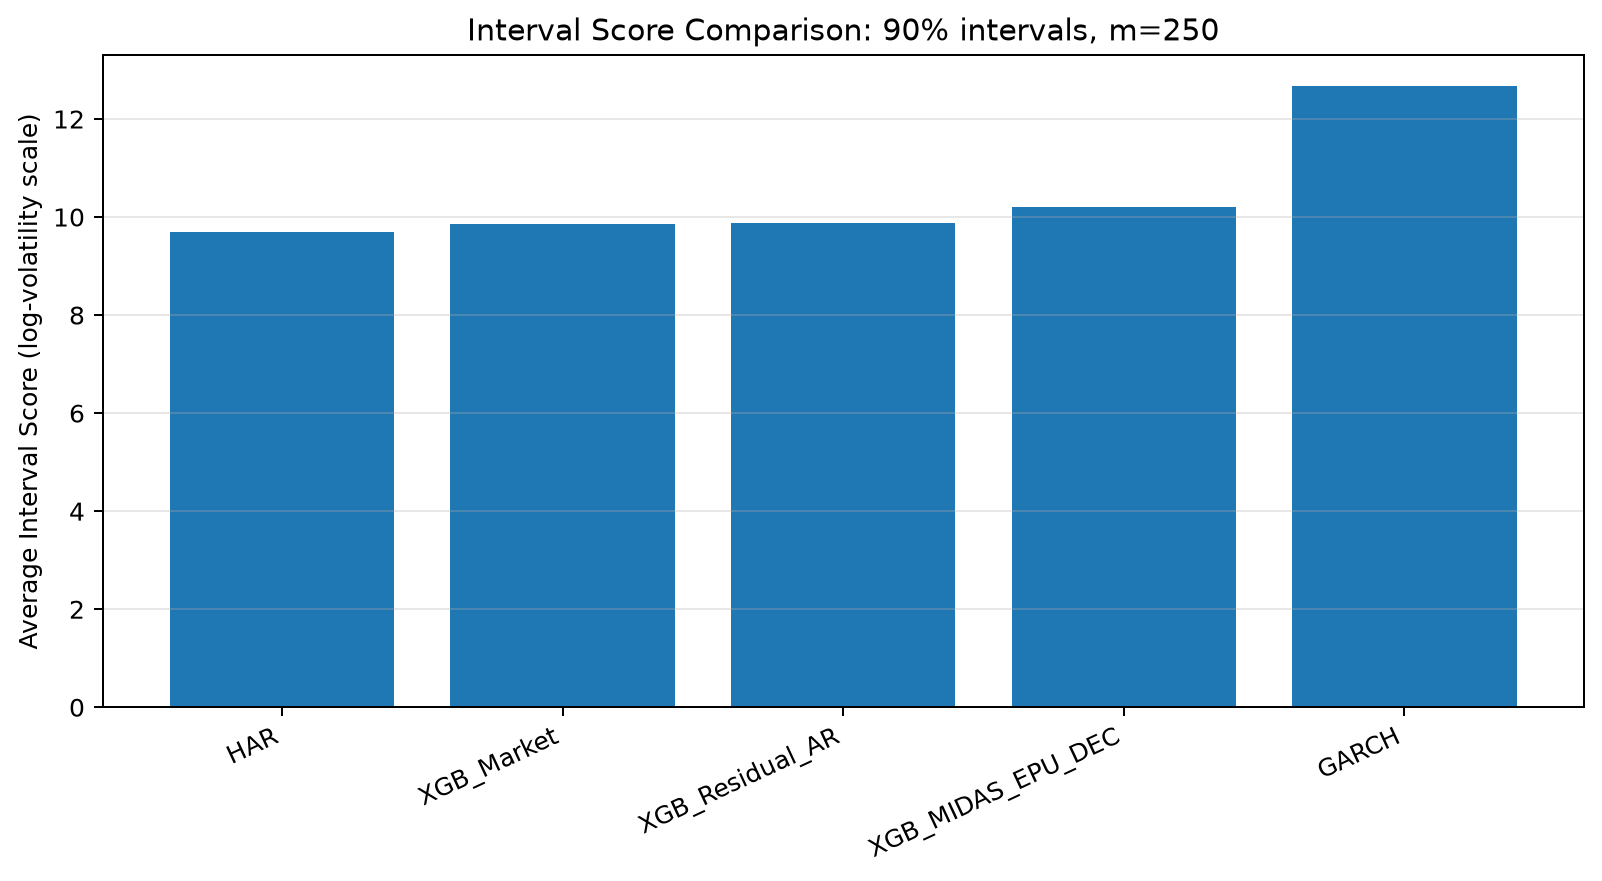
\includegraphics[width=.88\textwidth]{../../results/revised/intervals/fig_interval_score_main.png}
\caption{五模型共同日期上的区间得分}\label{fig:interval_score_main}\end{figure}
\begin{figure}[htbp]\centering
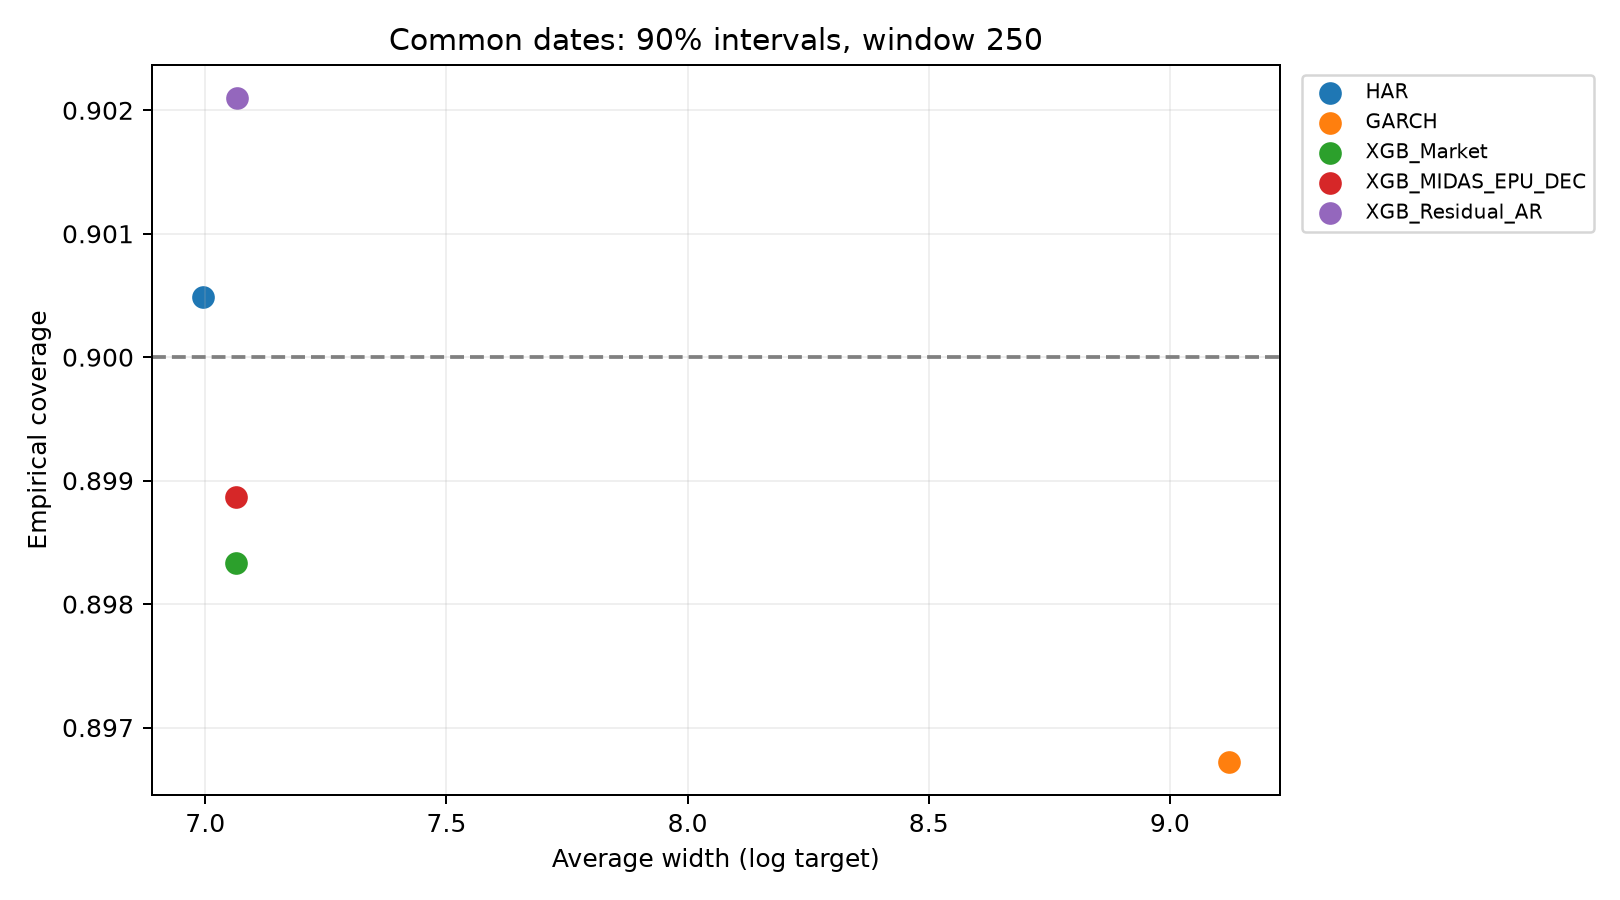
\includegraphics[width=.88\textwidth]{../../results/revised/intervals/fig_coverage_width_tradeoff_main.png}
\caption{共同日期上的覆盖率与区间宽度}\label{fig:coverage_width_tradeoff}\end{figure}

\subsection{覆盖检验及局部表现}
\begin{table}[htbp]\centering\caption{共同日期上的主设置覆盖诊断}\label{tab:christoffersen_main}
\begin{tabular}{lrrrr}\toprule
模型 & 违约数 & $p_{uc}$ & $p_{ind}$ & $p_{cc}$ \\
\midrule
HAR & 185 & 0.9445 & 0.1024 & 0.2629 \\
GARCH(1,1) & 192 & 0.6388 & 0.1370 & 0.2964 \\
XGB-Market & 189 & 0.8110 & 0.0987 & 0.2487 \\
XGB-AR & 182 & 0.7623 & 0.1896 & 0.4041 \\
DEC & 188 & 0.8712 & 0.0880 & 0.2303 \\
\bottomrule\end{tabular}\end{table}

主设置中五模型的UC、IND和CC参考检验均未在5\%水平拒绝。不拒绝不能证明正确覆盖，未对这些覆盖诊断进行多重检验调整。95\%区间、窗口120时，DEC的独立性$p=0.0062$、条件覆盖$p=0.0233$，仍提示违约聚集；不能只报告有利的主设置。

相邻60日覆盖窗口高度重叠。滚动覆盖率和近期区间路径仅展示样本动态，不能作为独立重复证据，也不能把全部未覆盖都归因于噪声或突然冲击。
\begin{figure}[htbp]\centering
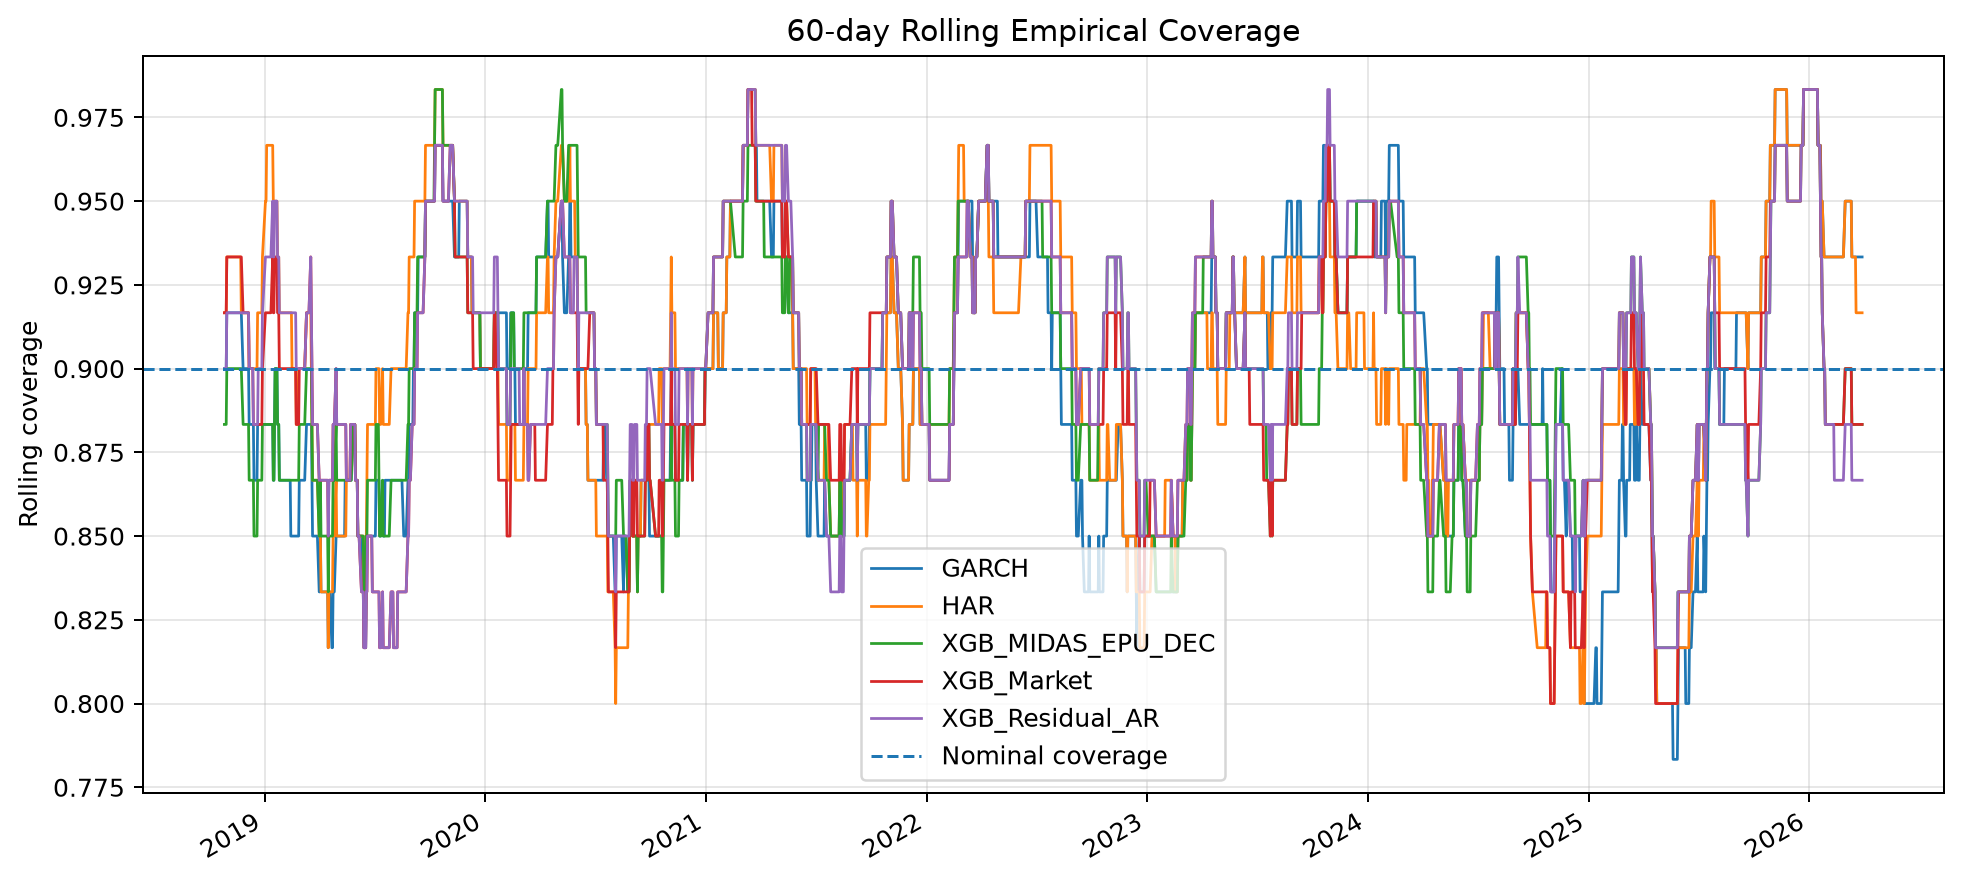
\includegraphics[width=.88\textwidth]{../../results/revised/intervals/fig_rolling_coverage_main.png}
\caption{共同评价段内60日滚动覆盖率}\label{fig:rolling_coverage}\end{figure}
\begin{figure}[htbp]\centering
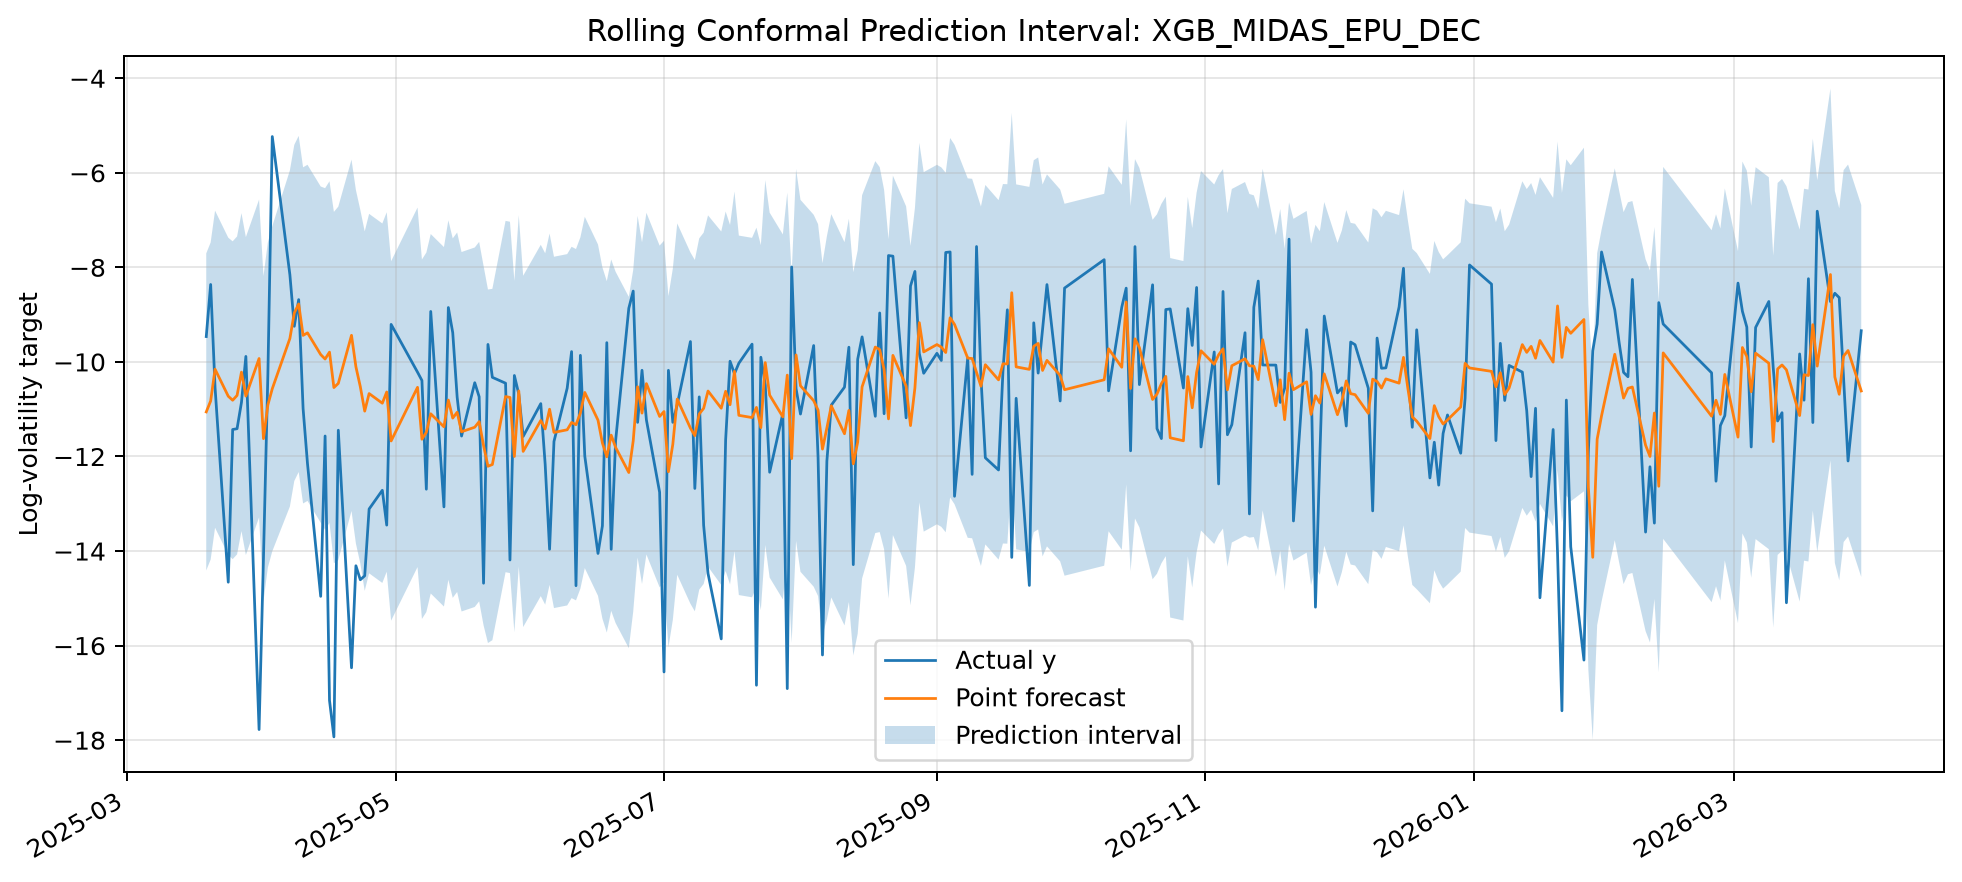
\includegraphics[width=.88\textwidth]{../../results/revised/intervals/fig_interval_series_XGB_MIDAS_EPU_DEC.png}
\caption{修订DEC的近期滚动残差区间}\label{fig:interval_series_xgb_midas}\end{figure}

\subsection{窗口与名义水平的敏感性}
\begin{table}[htbp]\centering\caption{共同日期上90\%区间的平均得分}\label{tab:interval_robustness}
\begin{tabular}{lrrr}\toprule 模型 & 窗口120 & 窗口250 & 窗口500\\\midrule
HAR & 9.7468 & 9.6973 & 9.6938\\
GARCH(1,1) & 12.6511 & 12.6634 & 12.6021\\
XGB-Market & 9.9336 & 9.8534 & 9.8528\\
XGB-AR & 9.9387 & 9.8793 & 9.8628\\
DEC & 10.2852 & 10.1995 & 10.1807\\
\bottomrule\end{tabular}\end{table}
六组名义水平与窗口设置、五模型共30组结果均随项目提供。排序和覆盖表现应按具体设置判断，不从单一主设置推广一般有效性。对CSI300而言，修订DEC的主设置得分由历史10.1991变为10.1995，略差；基准排序没有因数值修正而改变。

\subsection{本章小结}
修订DEC仍未改善XGB-Market及XGB-AR的区间质量。QLIKE改善与区间评分改善是不同命题；本文没有得到二者同时占优的证据。所有结论仅针对未来观测代理和本次滚动绝对残差构造，不能用于宣称潜在方差置信区间有效。
